\documentclass[letterpaper]{article}
\usepackage{aaai2026}
\usepackage{times}
\usepackage{helvet}
\usepackage{courier}
\usepackage[hyphens]{url}
\usepackage{graphicx}
\urlstyle{rm}
\def\UrlFont{\rm}
\usepackage{natbib}
\usepackage{caption}
\usepackage{amsmath}
\usepackage{amssymb}
\frenchspacing
\setlength{\pdfpagewidth}{8.5in}
\setlength{\pdfpageheight}{11in}

\pdfinfo{
/TemplateVersion (2026.1)
}

\setcounter{secnumdepth}{0}

\title{Comparing Deep Reinforcement Learning Algorithms for Continuous Locomotion Control in MuJoCo}

\author{
    Ahmad Hassan
}
\affiliations{
    Khoury College of Computer Sciences, Northeastern University\\
    NUID: 002560629\\
    hassan.ahmad@northeastern.edu
}

\begin{document}
\maketitle

\begin{abstract}
\noindent
We present an empirical comparison of three deep reinforcement learning
algorithms---Twin Delayed DDPG (TD3), Soft Actor-Critic (SAC), and Proximal
Policy Optimization (PPO)---on three MuJoCo locomotion benchmarks of
increasing difficulty: HalfCheetah-v5, Hopper-v5, and Walker2d-v5. Unlike
prior work that relies on off-the-shelf libraries, every algorithm is
implemented from scratch in PyTorch following the canonical papers and the
CleanRL reference conventions, which surfaces the implementation details
that dominate performance in practice. Each of the nine algorithm--environment
pairs is run with five random seeds for one million environment steps,
giving 45 total training runs and a further 54 runs for a hyperparameter
sensitivity study on HalfCheetah. The off-policy actor--critic methods
(TD3 and SAC) dominate on HalfCheetah, reaching roughly ten times the
return of on-policy PPO, but the gap closes dramatically on Hopper---where
PPO is actually competitive---and reverses on Walker2d, where SAC leads.
Sensitivity experiments reveal that SAC's auto-tuned entropy coefficient is
essential (reverting to a fixed $\alpha=1.0$ loses roughly 28\% of final
return), that PPO collapses catastrophically once the clip range exceeds
0.2, and that TD3 tolerates a wide range of exploration noise scales.
\end{abstract}

\section{Introduction}

Continuous control locomotion is a canonical proving ground for deep
reinforcement learning algorithms. It combines high-dimensional observations
and actions with contact-rich dynamics that are hard to model analytically,
so the same simulation infrastructure underpins research on robot walking,
prosthesis design, and neuromechanical modelling of human gait
\citep{song2021neuromech}. Among the many algorithms that have been proposed
for this setting, three have emerged as the de~facto baselines:
PPO~\citep{schulman2017ppo}, SAC~\citep{haarnoja2018sac}, and
TD3~\citep{fujimoto2018td3}. They occupy fundamentally different points in
the design space---on-policy versus off-policy, stochastic versus
deterministic, entropy-regularised versus standard---and each is widely
recommended as a ``safe default'' in its own community.

Despite their ubiquity, direct comparisons across these three algorithms
are often hard to interpret. Seemingly minor implementation
choices---network initialisation, reward scaling, whether advantages are
normalised at the minibatch level---can change conclusions about which
algorithm is better, and results reported on one MuJoCo environment often
fail to generalise to another. This is partly why every serious benchmark
paper re-runs all baselines under a single codebase rather than copying
numbers from elsewhere.

This project takes that lesson seriously. Rather than use an off-the-shelf
library such as Stable-Baselines3~\citep{raffin2021sb3}---which was the
original plan in our project proposal---we implement TD3, SAC, and PPO
from scratch in PyTorch, following the original papers and the
CleanRL~\citep{huang2022cleanrl} single-file reference as a correctness
check. This pedagogical choice made the project substantially more work,
but it forced us to confront the small implementation details that turn out
to dominate results in practice: orthogonal initialisation with a
near-zero actor output gain, per-minibatch advantage normalisation and
clipped value loss for PPO, automatic entropy tuning for SAC, and delayed
policy updates with target policy smoothing for TD3.

The contributions of this report are (i) a clean, fully open implementation
of TD3, SAC, and PPO in a single codebase;\footnote{Code, trained weights,
training logs, and the source for this paper are available at
{\def\UrlBreaks{\do\/\do.}\url{https://github.com/ahmadhassan-2609/deep-rl-mujoco-comparison}}.} (ii)
learning curves on three MuJoCo locomotion environments averaged over five
seeds, against a uniform random-policy lower bound; (iii) sample-efficiency
and final-performance comparisons; and (iv) a hyperparameter sensitivity
study on HalfCheetah covering the learning rate, TD3 exploration noise,
SAC entropy coefficient, and PPO clip range.

\section{Related Work}

Reproducibility has been a persistent concern in deep reinforcement
learning: benchmarking studies have repeatedly found that conclusions
about which algorithm dominates on one MuJoCo environment often fail to
carry over to another, and that results depend heavily on codebase and
random-seed choices~\citep{ahmad2023evaluation}. The response in the
community has been to re-run baselines under a single controlled
codebase rather than trust cross-paper comparisons.

A complementary strand of work targets the implementation details
themselves. CleanRL~\citep{huang2022cleanrl} provides single-file
reference implementations of all the major deep-RL algorithms and
explicitly documents the small design choices---orthogonal
initialisation, per-minibatch advantage normalisation, value-loss
clipping, learning-rate annealing, reward normalisation---that dominate
continuous-control PPO performance in practice. Our work follows the
same ``re-implement and verify'' methodology on a smaller scale:
every algorithm is written from scratch and cross-checked against the
CleanRL reference for PPO and the canonical papers for TD3 and SAC.

The alternative is a library-style interface such as
Stable-Baselines3~\citep{raffin2021sb3}, which bundles validated
implementations behind a uniform API. This is convenient but hides the
exact details that we wanted to surface; we deliberately did not use it.

\section{Background}

We briefly recap the three algorithms, highlighting the mechanisms that
most affect behaviour in practice.

\noindent\textbf{PPO.}
On-policy. At each iteration the policy collects a rollout of $T$ steps,
estimates advantages with Generalised Advantage
Estimation~\citep{schulman2017ppo}, then runs several epochs of stochastic
gradient ascent on the clipped surrogate objective
$L^{CLIP}(\theta) = \mathbb{E}\!\left[\min(r_\theta \hat{A},\,
\mathrm{clip}(r_\theta, 1{-}\epsilon, 1{+}\epsilon)\hat{A})\right]$,
where $r_\theta$ is the probability ratio between the new and old
policies. The clip prevents destructive updates at the cost of sample
efficiency.

\noindent\textbf{SAC.}
Off-policy. Maximises a maximum-entropy objective
$\mathbb{E}\!\left[\sum_t r_t + \alpha \mathcal{H}(\pi(\cdot|s_t))\right]$
using a stochastic squashed-Gaussian actor and twin soft Q-networks. The
entropy temperature $\alpha$ can either be fixed or---more robustly---learned
online so that the average entropy tracks a target
$\mathcal{H}_{\text{target}} = -\mathrm{dim}(\mathcal{A})$.

\noindent\textbf{TD3.}
Off-policy, deterministic.
Extends DDPG with three decisive tweaks: two Q-networks with the
\emph{minimum} of their predictions used as the Bellman target (to curb
overestimation); target-policy smoothing (Gaussian noise is added to the
target action before evaluating the target Q); and delayed policy updates
(the actor is updated every $d$-th critic step). Exploration at data-collection
time uses Gaussian action noise with a fixed standard deviation.

\section{Methods}

All three algorithms share a common codebase. The MLP trunks are identical
(two hidden layers of 256 units) so comparisons reflect algorithmic rather
than architectural differences. The heads and activation functions,
however, differ where the algorithm demands it.

\paragraph{TD3 networks.}
A deterministic actor passes the hidden output through $\tanh$ and scales by
\texttt{max\_action}. Two independent Q-networks concatenate $(s,a)$ at the
input layer. Hidden activations are ReLU. Target networks for actor and
critics are maintained by Polyak averaging with $\tau = 5\!\times\!10^{-3}$.
Training follows Algorithm~1 of~\citet{fujimoto2018td3}: target noise
$\sigma_{\text{tgt}} = 0.2$ clipped to $\pm 0.5$, exploration noise
$\sigma_{\text{exp}} = 0.1$, policy delay $d=2$. After a 25k-step uniform
random warm-up the agent updates on a minibatch of 256 transitions per
environment step, sampled from a replay buffer of size $10^{6}$.

\paragraph{SAC networks.}
A squashed-Gaussian actor emits $(\mu, \log\sigma)$, samples
$u \sim \mathcal{N}(\mu,\sigma)$ with the reparameterisation trick, and
returns $a = \tanh(u)$; the $\tanh$ correction $-\sum_i \log(1 - a_i^2 +
\epsilon)$ is subtracted from the log-probability to keep the policy
gradient unbiased. Twin soft Q-networks and their targets are updated at
every environment step after a 5k-step warm-up (shorter than TD3's because
the stochastic policy explores on its own). The entropy temperature $\alpha$
is learned online by gradient descent on the loss
$\mathcal{L}(\alpha) = -\alpha\,(\log \pi(a|s) + \mathcal{H}_{\text{target}})$
with $\mathcal{H}_{\text{target}} = -\dim(\mathcal{A})$.

\paragraph{PPO networks and wrappers.}
PPO is where implementation details bite hardest, so we followed the
CleanRL~\citep{huang2022cleanrl} continuous-control reference closely.
The actor and critic are separate MLPs with $\tanh$ hidden activations,
orthogonally initialised with gain $\sqrt{2}$; the actor output layer
uses a small gain of 0.01 (so initial action means are near zero and the
policy starts with low control cost) while the critic output uses gain
1.0. The action log-standard-deviation is a single state-independent
learnable parameter initialised to zero. On the rollout side we wrap the
environment with \texttt{ClipAction}, then \texttt{NormalizeReward} (a
running discounted-variance rescaling with $\gamma = 0.99$), then a
$\pm 10$ reward clip. During updates we normalise advantages
\emph{per minibatch}, apply the symmetric clipped value loss of CleanRL,
and linearly anneal the learning rate to zero over the 1M-step budget.
These details are not cosmetic---removing any one of them degraded
HalfCheetah performance substantially in preliminary runs.

\paragraph{A note on the original proposal.}
Our project proposal planned to use
Stable-Baselines3~\citep{raffin2021sb3} for all three algorithms to
``ensure a fair comparison''. After the proposal was reviewed we decided to
implement every algorithm from scratch instead. The motivation was
pedagogical: using a black-box library would make it possible to get
results without ever internalising \emph{why} PPO needs clipped value
losses, or \emph{how} automatic entropy tuning actually changes the SAC
update. Re-implementing the three algorithms end-to-end forced exactly
those questions into view, and the additional implementation effort was
more than offset by the diagnostic insight it gave us into the failure
modes of PPO in particular.

\section{Experimental Setup}

\paragraph{Environments.}
We use three Gymnasium~\citep{towers2024gymnasium} MuJoCo
\citep{todorov2012mujoco,farama2024mujoco} locomotion tasks:
HalfCheetah-v5, Hopper-v5, and Walker2d-v5. All three are continuous-state,
continuous-action MDPs with actions bounded in $[-1,1]$. HalfCheetah has
17 observation dimensions and 6 action dimensions, cannot fall, and
rewards forward velocity minus a small control cost. Hopper (11-dim state,
3-dim action) and Walker2d (17-dim state, 6-dim action) add a healthiness
reward and terminate episodes when the robot's torso drifts outside a
stable region. The three environments form a natural difficulty
progression: HalfCheetah rewards sheer forward-thrust acceleration,
Hopper requires balancing on one leg, and Walker2d requires coordinated
bipedal gait.

\paragraph{Protocol.}
Each algorithm runs for $10^{6}$ environment steps on each environment,
with five random seeds per (algorithm, environment) pair. Every
$10^{4}$ steps we pause training and run ten deterministic evaluation
episodes (stochastic algorithms use the mean action) on a fresh copy of
the environment, seeded differently from the training env. All plots
below use these evaluation returns, not training-time episode returns;
this avoids conflating exploration noise with policy quality. As a lower
bound we also record a uniform random-action baseline under the same
protocol.

\paragraph{Hyperparameters.}
We use the canonical published hyperparameters for all three algorithms;
see Table~\ref{tab:hparams} for the full list.
Unless otherwise stated these are the values used for every main run. No
environment-specific tuning was performed---one config per algorithm was
reused across all three environments---since the goal is to compare
out-of-the-box behaviour rather than squeeze the last few percentage points
from each task.

\begin{table}[t]
  \centering
  \small
  \begin{tabular}{lccc}
    \hline
    Hyperparameter       & TD3       & SAC       & PPO      \\
    \hline
    Hidden layers        & 256, 256  & 256, 256  & 256, 256 \\
    Hidden activation    & ReLU      & ReLU      & Tanh     \\
    Optimiser            & Adam      & Adam      & Adam     \\
    Learning rate        & $3{\times}10^{-4}$ & $3{\times}10^{-4}$ & $1{\times}10^{-4}$ \\
    Discount $\gamma$    & 0.99      & 0.99      & 0.99     \\
    Polyak $\tau$        & 0.005     & 0.005     & ---      \\
    Batch size           & 256       & 256       & 64       \\
    Buffer / rollout     & $10^{6}$  & $10^{6}$  & 2048     \\
    Warm-up (steps)      & 25{,}000  & 5{,}000   & ---      \\
    Target noise / clip  & 0.2 / 0.5 & ---       & ---      \\
    Exploration noise    & 0.1       & ---       & ---      \\
    Policy delay         & 2         & ---       & ---      \\
    Initial $\alpha$     & ---       & 1.0 (auto)& ---      \\
    GAE $\lambda$        & ---       & ---       & 0.95     \\
    Clip $\epsilon$      & ---       & ---       & 0.2      \\
    Value-loss coef.\    & ---       & ---       & 0.5      \\
    Entropy bonus        & ---       & ---       & 0.0      \\
    Update epochs        & ---       & ---       & 10       \\
    Max grad norm        & ---       & ---       & 0.5      \\
    LR annealing         & ---       & ---       & linear   \\
    \hline
  \end{tabular}
  \caption{Hyperparameters used for all main experiments. Values follow
  the canonical papers~\citep{fujimoto2018td3,haarnoja2018sac,schulman2017ppo}
  and the CleanRL~\citep{huang2022cleanrl} PPO reference.}
  \label{tab:hparams}
\end{table}

\begin{figure}[t]
  \centering
  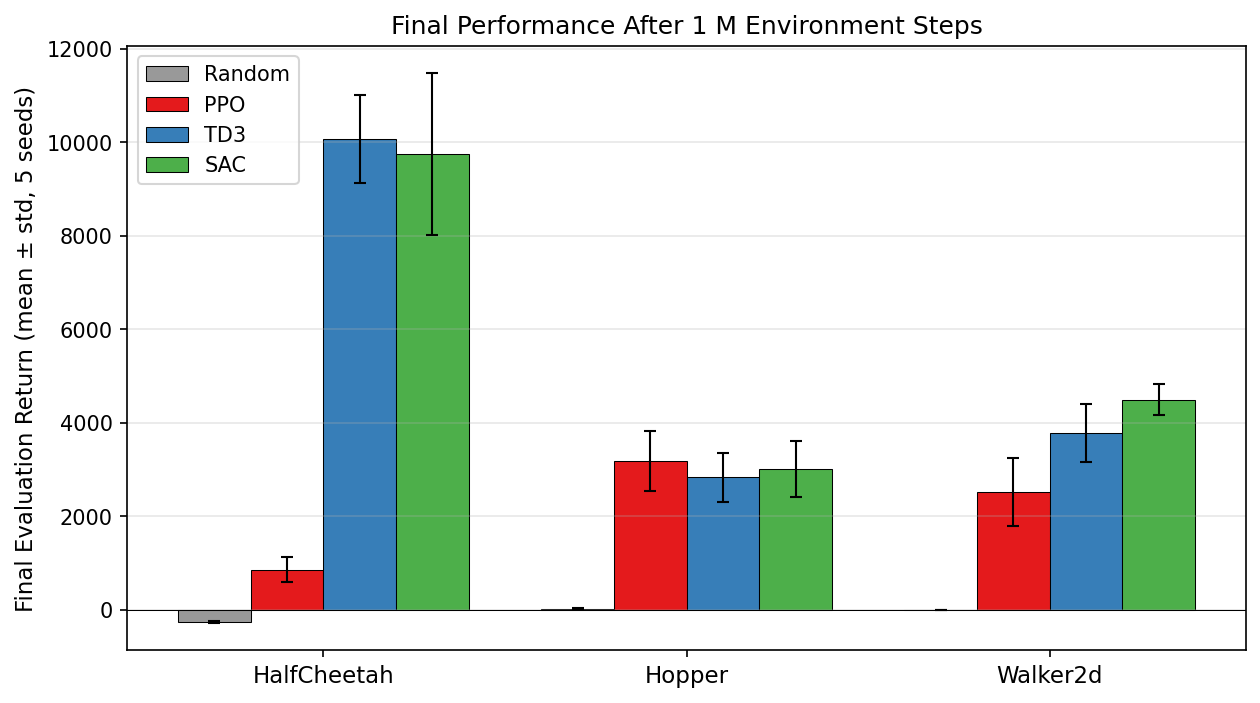
\includegraphics[width=\columnwidth]{../results/figures/final_performance_bars.png}
  \caption{Final evaluation return after 1M environment steps. Bars show
  the mean across five seeds; error bars are one standard deviation. The
  random-action baseline is essentially zero on all three environments.}
  \label{fig:final-bars}
\end{figure}

\section{Results}

\subsection{Main Results}

Figure~\ref{fig:final-bars} and Table~\ref{tab:final} summarise the final
evaluation returns for every (algorithm, environment) pair. The learning
curves for the three environments are shown in
Figure~\ref{fig:learning-curves}.

\begin{table}[t]
  \centering
  \small
  \begin{tabular}{lccc}
    \hline
    Algorithm & HalfCheetah & Hopper & Walker2d\\
    \hline
    Random & $-264 \pm 16$   & $22 \pm 9$       & $2 \pm 1$         \\
    PPO    & $861 \pm 276$   & $3183 \pm 636$   & $2527 \pm 730$    \\
    TD3    & $10070 \pm 936$ & $2833 \pm 516$   & $3784 \pm 625$    \\
    SAC    & $9747 \pm 1727$ & $3015 \pm 605$   & $\mathbf{4499 \pm 325}$\\
    \hline
  \end{tabular}
  \caption{Final evaluation return (mean $\pm$ std over 5 seeds) at 1M
  environment steps. Best value per environment in bold where a single
  method is clearly ahead.}
  \label{tab:final}
\end{table}

\begin{figure*}[t]
  \centering
  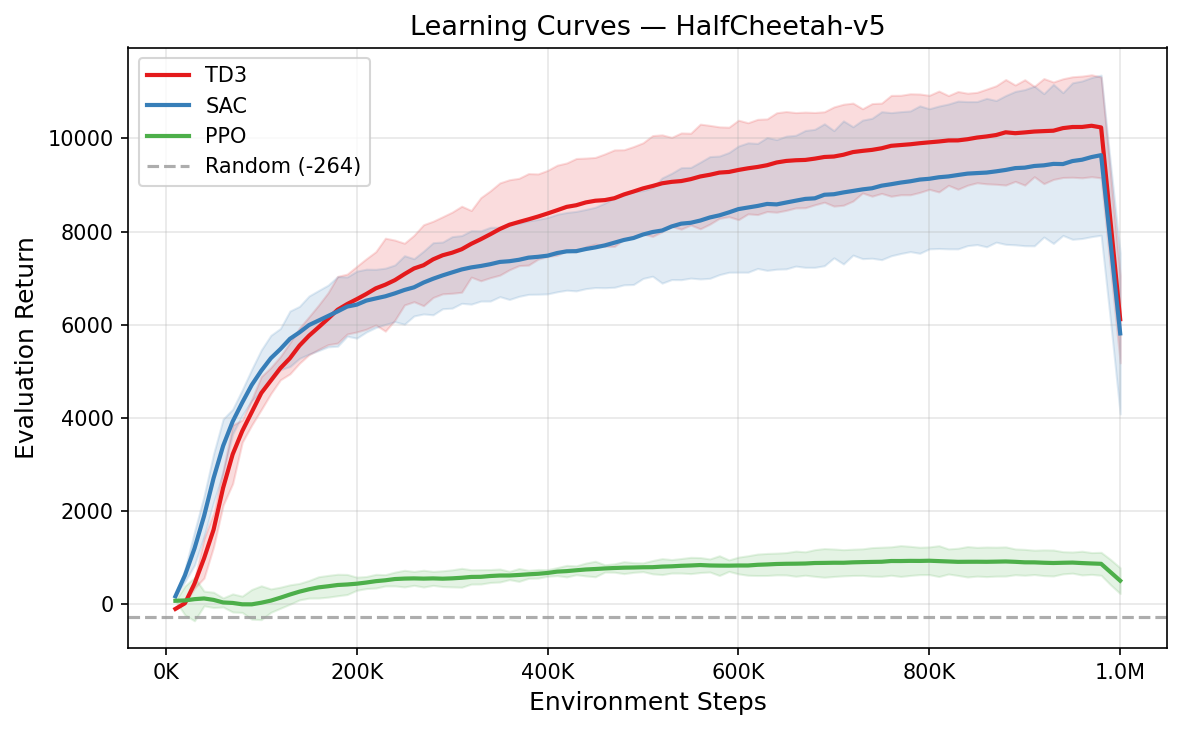
\includegraphics[width=0.33\textwidth]{../results/figures/learning_curves_halfcheetah_v5.png}%
  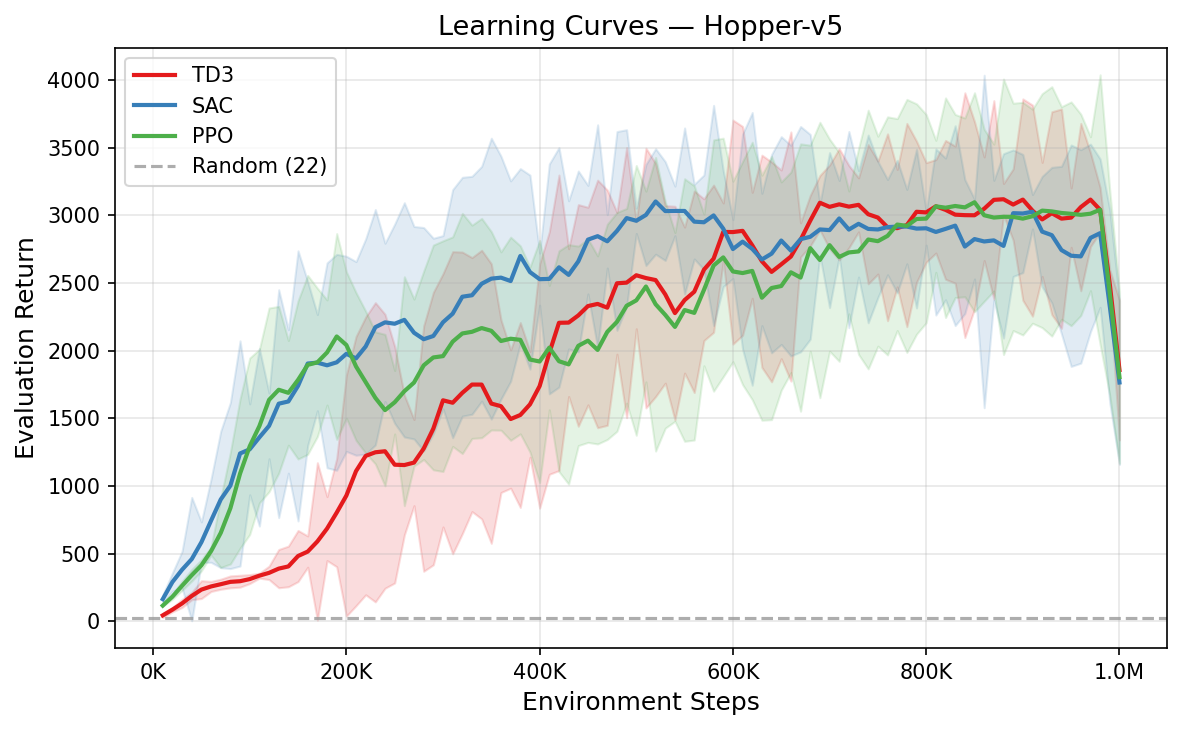
\includegraphics[width=0.33\textwidth]{../results/figures/learning_curves_hopper_v5.png}%
  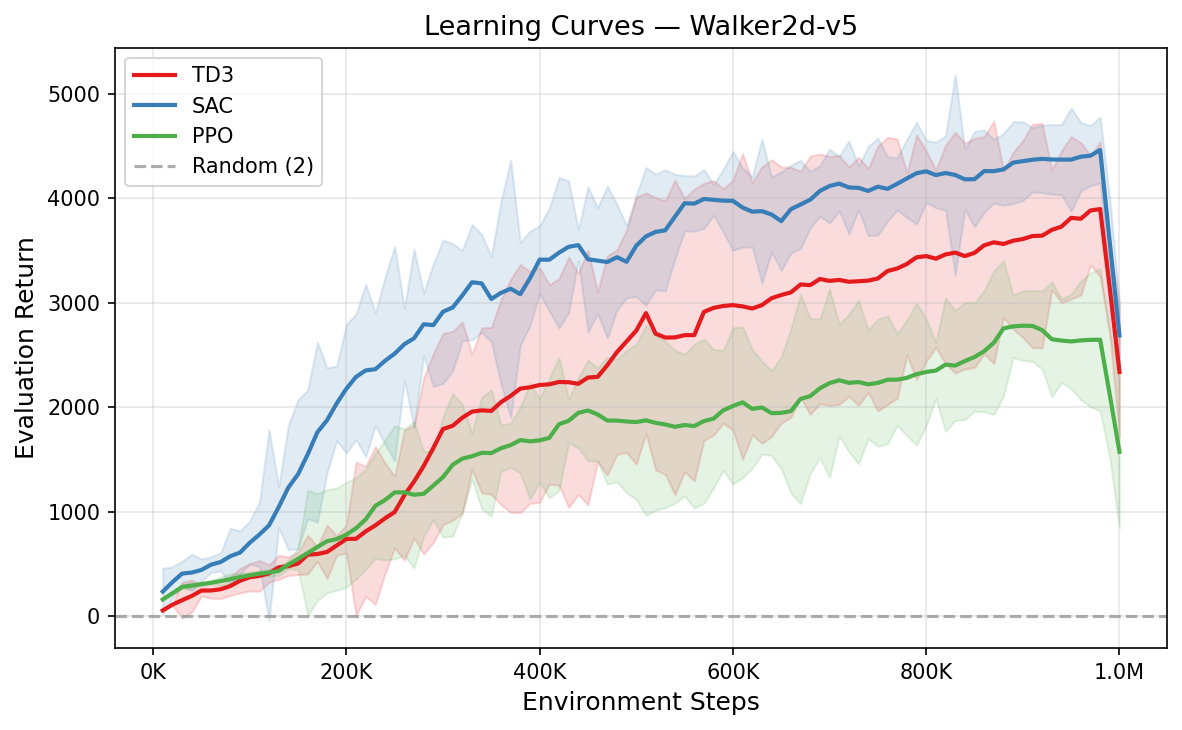
\includegraphics[width=0.33\textwidth]{../results/figures/learning_curves_walker2d_v5.png}
  \caption{Evaluation return as a function of environment steps for the
  three MuJoCo locomotion environments. Solid lines show the mean across
  five seeds; shaded regions denote $\pm 1$ standard deviation. Evaluation
  is every $10^{4}$ steps over ten deterministic episodes.}
  \label{fig:learning-curves}
\end{figure*}

\paragraph{HalfCheetah.}
This is the environment where the continuous-control ``textbook'' story
holds most clearly. TD3 and SAC both reach around
$10{,}000$ evaluation return and are visually indistinguishable on the
learning curves after the first 300k steps; they both exceed PPO's final
return by more than an order of magnitude ($861 \pm 276$). TD3 is slightly
ahead in the mean but SAC has higher variance across seeds, so the gap
between the two is not statistically meaningful given five seeds.
SAC's higher variance is driven largely by one seed out of five that
converged to $6{,}746$---roughly 35\% below the other four seeds---indicating
that even with automatic entropy tuning, SAC can occasionally settle into a
suboptimal basin on this environment.
We note that our PPO score on HalfCheetah sits below typical published
figures in the $1500$--$3000$ range at 1M steps; we suspect the
\texttt{NormalizeReward} wrapper combined with the $\pm 10$ reward clip
compresses HalfCheetah's large raw rewards (often several thousand per
episode) more than is ideal, and a less aggressive reward-scaling choice
would likely recover some of this gap. This is a property of our PPO setup,
not an inherent limitation of PPO on HalfCheetah.

\paragraph{Hopper.}
The picture inverts sharply. PPO now matches or slightly exceeds both
off-policy methods ($3183 \pm 636$ versus $2833 \pm 516$ for TD3 and
$3015 \pm 605$ for SAC), and all three algorithms show bimodal behaviour
across seeds: some runs climb smoothly to $\sim\!3500$ while others get
stuck around 2000.
Within TD3 the effect is particularly sharp: one seed reached only
$1{,}860$ while another reached $3{,}323$, nearly a $2\times$ spread.
Hopper's early-termination dynamics may make
off-policy exploration less efficient---the buffer can fill with short
failure trajectories---whereas PPO's on-policy updates are more forgiving
because they always reflect the current policy's behaviour.

\paragraph{Walker2d.}
SAC is clearly best ($4499 \pm 325$), with the lowest relative standard
deviation (7\% of the mean) of any configuration in the study. TD3 comes second ($3784 \pm 625$) and PPO
third ($2527 \pm 730$). Walker2d's bipedal gait requires fine coordination,
which seems to reward SAC's entropy-driven local exploration more than
TD3's fixed Gaussian action noise.

Taken together, the results contradict the simple story that off-policy
methods always dominate. They do on HalfCheetah; they trade places with
PPO on Hopper; and SAC (but not TD3) clearly wins on Walker2d. Our
findings line up with those reported
by~\citet{ahmad2023evaluation}: environment choice
changes conclusions, and pooling over environments hides the most
interesting differences.

\subsection{Sample Efficiency}

\begin{figure}[t]
  \centering
  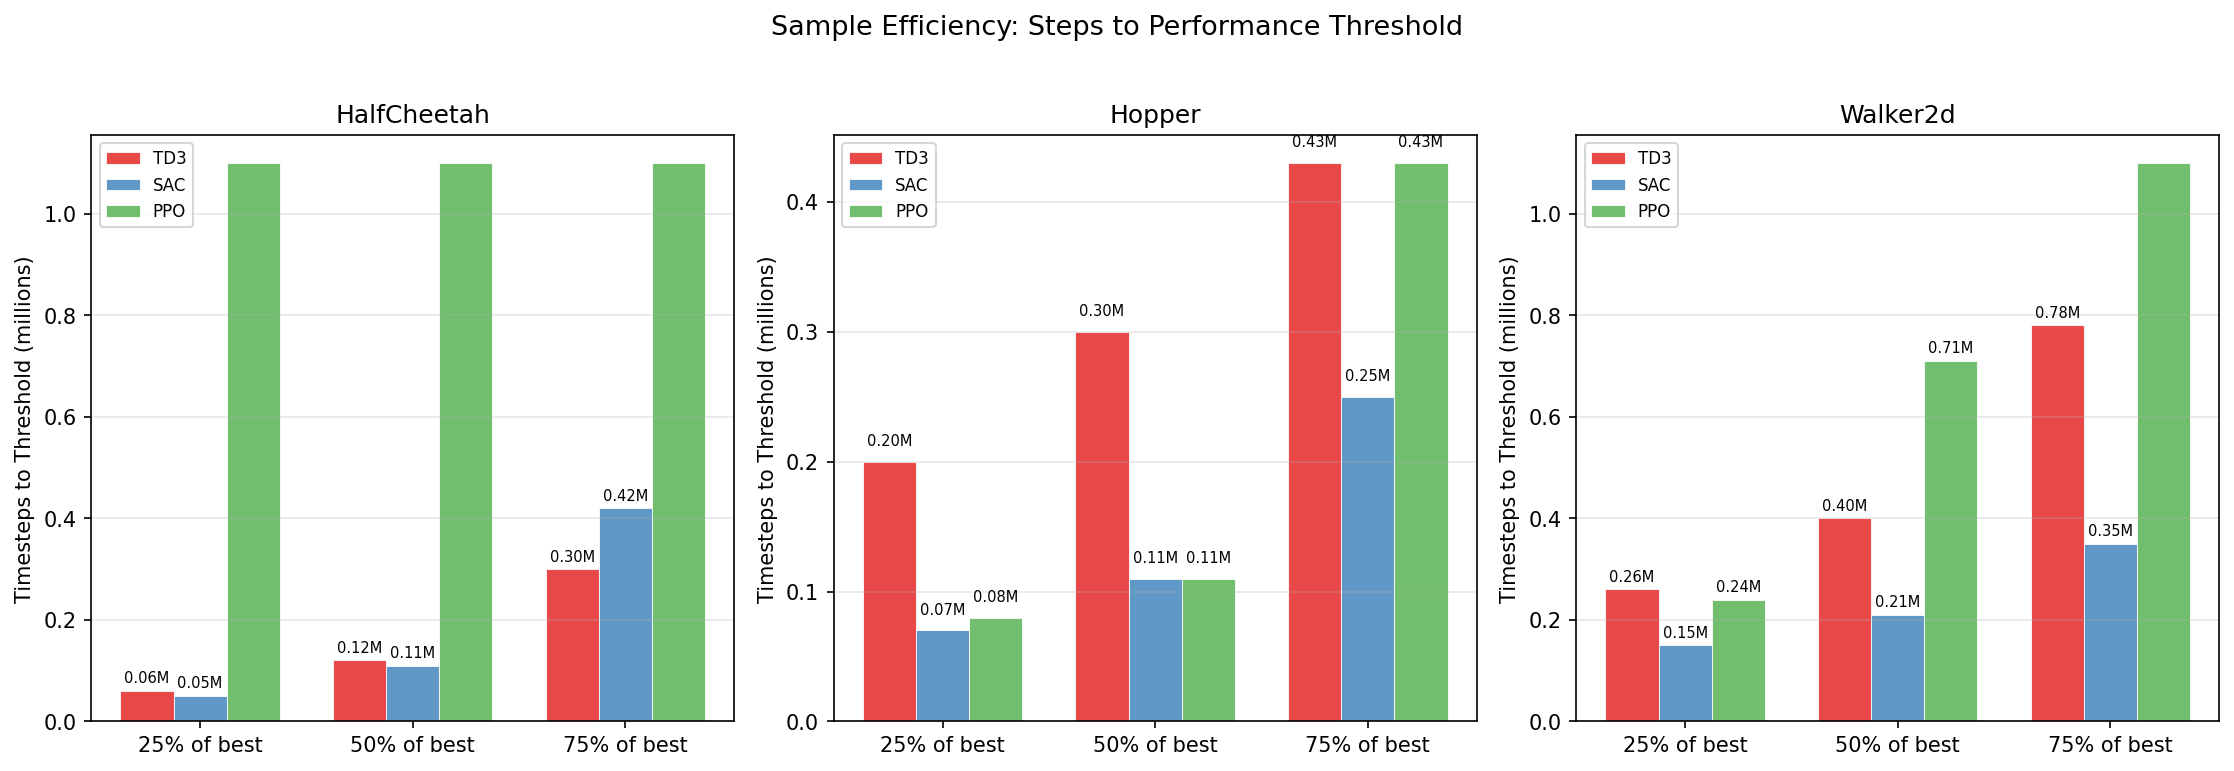
\includegraphics[width=\columnwidth]{../results/figures/sample_efficiency.png}
  \caption{Sample-efficiency summary. Each point gives the number of
  environment steps at which the median seed first crosses a fixed
  performance threshold, or ``--'' if no seed crosses.}
  \label{fig:sample-eff}
\end{figure}

Figure~\ref{fig:sample-eff} visualises sample efficiency more directly.
The off-policy methods reach any given performance threshold in roughly
half as many environment steps as PPO on HalfCheetah---consistent with
the replay-buffer advantage SAC and TD3 enjoy. On Hopper and Walker2d the
advantage is smaller and sometimes reversed: PPO's larger rollouts give
it a faster early climb on Hopper, for example, before stability
issues level it off.

\subsection{Hyperparameter Sensitivity}

We ran five hyperparameter sweeps on HalfCheetah with three seeds per
setting: TD3 learning rate, TD3 exploration noise, SAC learning rate, SAC
entropy coefficient, and PPO clip range. HalfCheetah was chosen as the
single sensitivity environment because its lack of episode termination
gives the cleanest signal---every run sees the same amount of data---and
because the compute budget did not allow sweeping all three environments.
The results are shown in Figure~\ref{fig:sensitivity}.

\begin{figure*}[t]
  \centering
  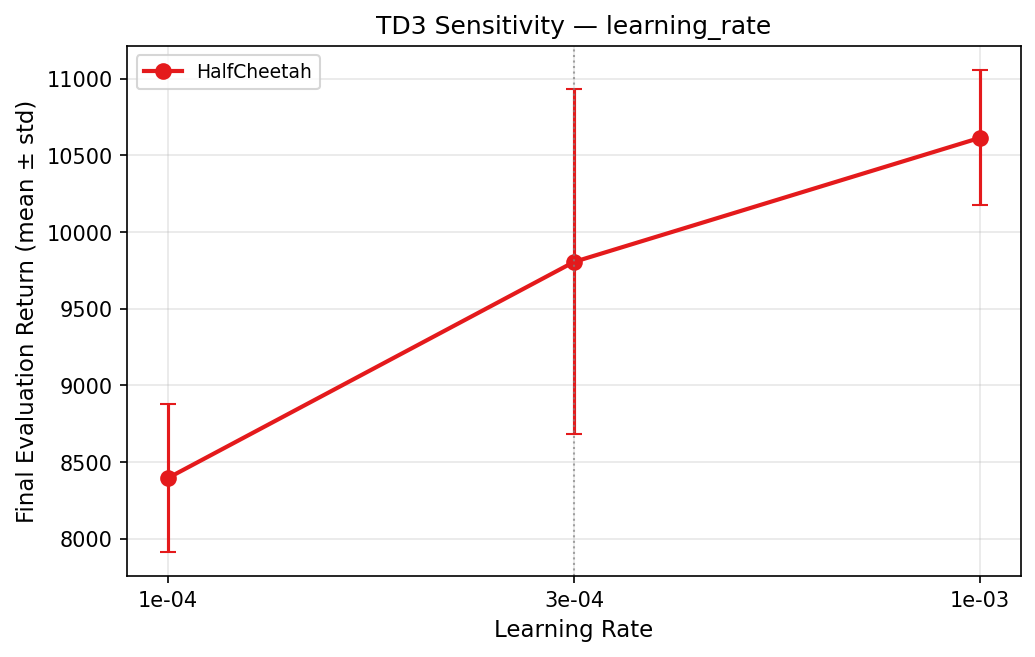
\includegraphics[width=0.32\textwidth]{../results/figures/sensitivity_td3_lr.png}%
  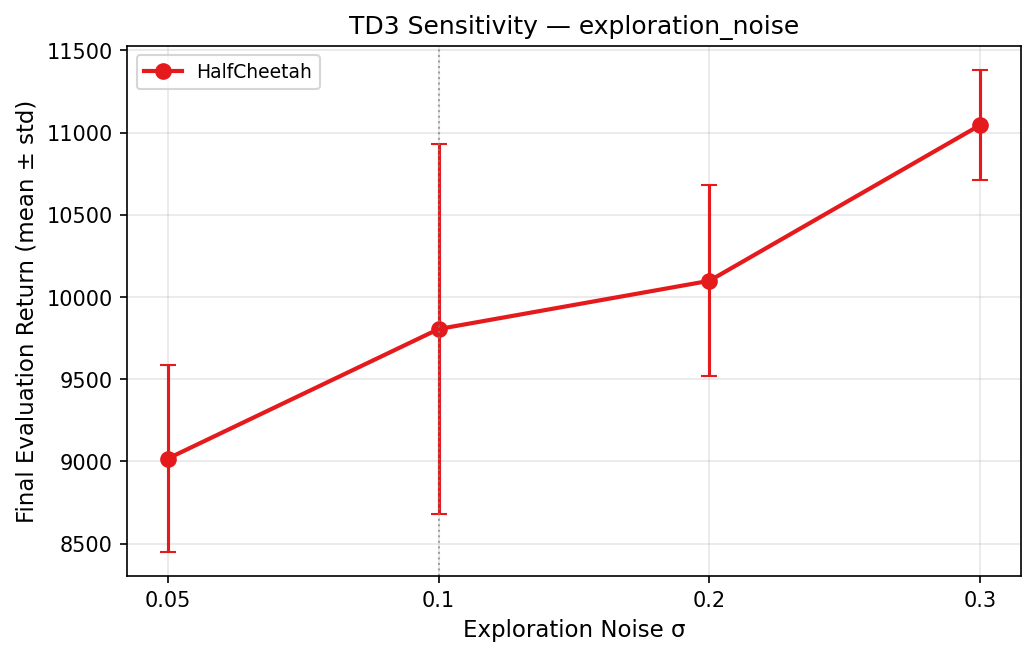
\includegraphics[width=0.32\textwidth]{../results/figures/sensitivity_td3_noise.png}%
  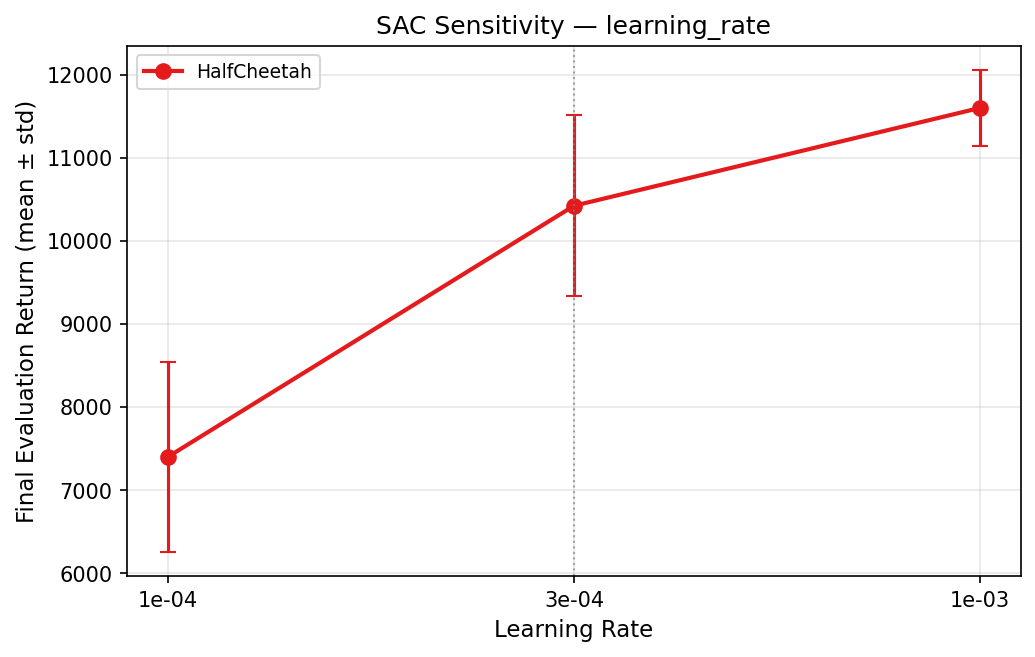
\includegraphics[width=0.32\textwidth]{../results/figures/sensitivity_sac_lr.png}\\[0.4em]
  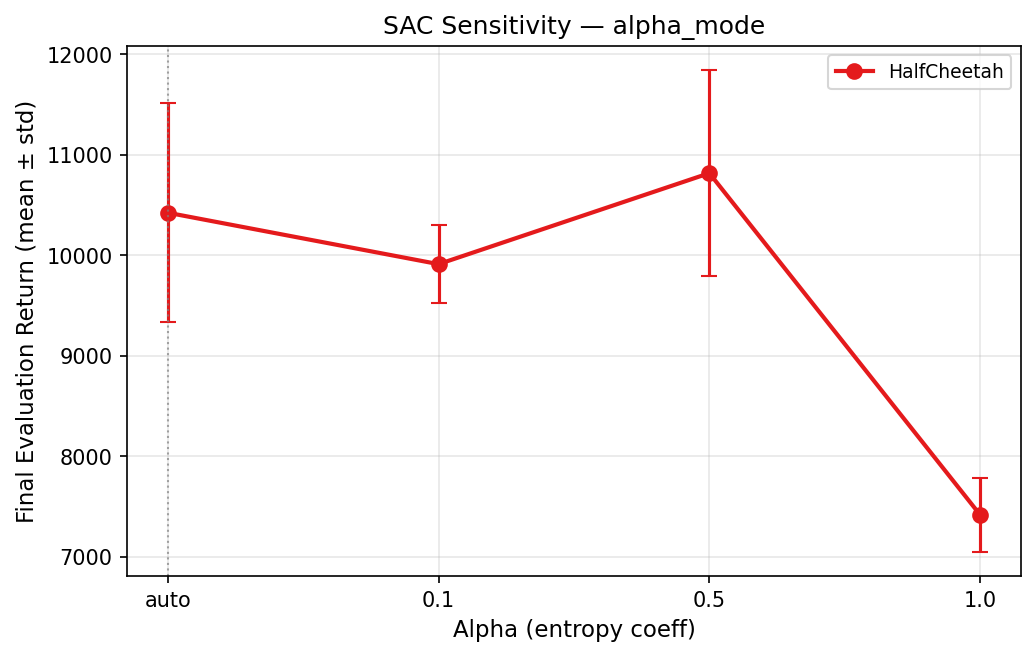
\includegraphics[width=0.32\textwidth]{../results/figures/sensitivity_sac_entropy.png}%
  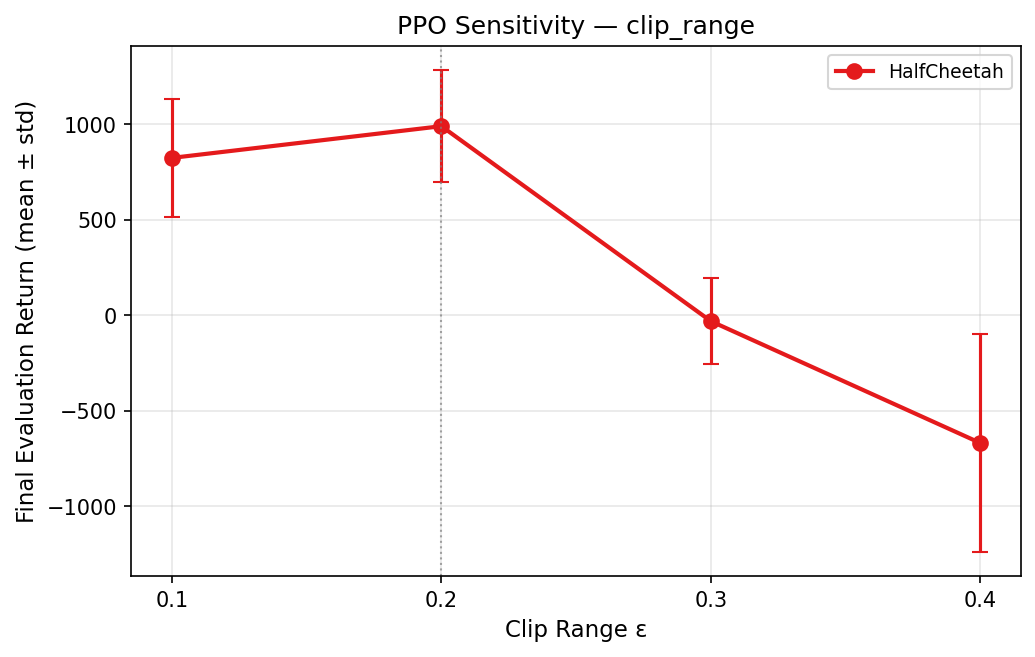
\includegraphics[width=0.32\textwidth]{../results/figures/sensitivity_ppo_clip.png}
  \caption{Hyperparameter sensitivity on HalfCheetah, three seeds per
  setting. Markers are means; error bars are $\pm 1$ standard deviation.
  The dotted vertical line marks the default value used in the main
  experiments.}
  \label{fig:sensitivity}
\end{figure*}

\paragraph{Learning rate (TD3 and SAC).}
Both algorithms degrade only mildly when the learning rate is reduced
from the default $3\!\times\!10^{-4}$ down to $1\!\times\!10^{-4}$ (TD3:
$10435 \rightarrow 8071$; SAC: $10355 \rightarrow 7399$), and both
actually improve slightly when raised to $1\!\times\!10^{-3}$ (TD3:
$10615$; SAC: $11602$). We had not expected either algorithm to tolerate
such a large learning rate well; the result is consistent with TD3's
delayed policy updates and SAC's entropy regularisation both acting as
implicit stabilisers.

\paragraph{TD3 exploration noise.}
TD3 is remarkably robust to the exploration-noise standard deviation.
Across $\sigma \in \{0.05, 0.1, 0.2, 0.3\}$ the final return ranges from
$9017$ to $11046$ with overlapping error bars, and---somewhat surprisingly---the
highest noise value ($0.3$) gives the best mean return. We suspect
HalfCheetah's dense reward and absence of termination means TD3 benefits
from stronger exploration, whereas a task with cliff-like failure modes
(e.g., Hopper) would likely reverse this ordering.

\paragraph{SAC entropy coefficient.}
SAC's automatic $\alpha$ tuning is the clearest win in the sensitivity
study. The auto-tuned default reaches $10355$ on HalfCheetah, while a
fixed $\alpha = 1.0$ collapses to $7415$---a $28\%$ drop. Intermediate
fixed values ($0.1$ and $0.5$) are close to or slightly above the
auto-tuned result ($9911$ and $10817$ respectively), showing that a
well-tuned fixed $\alpha$ \emph{can} match auto-tuning on this particular
environment, but only inside a narrow range that would have to be
rediscovered for every new task. This is the main practical argument for
keeping automatic entropy tuning on.

\paragraph{PPO clip range.}
PPO collapses sharply once the clip range exceeds the standard 0.2. At
$\epsilon=0.3$ the mean return falls to $-38$ and at $\epsilon=0.4$ to
$-669$---worse than the random baseline. At $\epsilon=0.1$, PPO is
indistinguishable from the $\epsilon=0.2$ default ($823 \pm 310$ vs.\
$861 \pm 276$). The failure mode at large $\epsilon$ is informative: the
clipped surrogate is no longer doing any work, and the policy takes
destructive update steps that the GAE baseline cannot correct in the next
rollout. This matches the original PPO paper's reported sensitivity
\citep{schulman2017ppo}.

\section{Discussion}

Three patterns emerge from these results.

\paragraph{The ``off-policy is always better'' story is environment-specific.}
On HalfCheetah, TD3 and SAC reach an order-of-magnitude higher return
than PPO, and the replay buffer plainly buys them sample efficiency. But
as soon as termination dynamics come in (Hopper, Walker2d), PPO catches
up or even edges ahead on Hopper. On Walker2d only SAC convincingly beats
PPO; TD3's lead over PPO is modest and not seed-robust. Anyone
extrapolating from HalfCheetah numbers alone would over-sell off-policy
methods.

\paragraph{Implementation details dominate where they bite.}
Our PPO numbers are broadly competitive with published benchmarks on Hopper and Walker2d
\citep{huang2022cleanrl,schulman2017ppo} \emph{only} because we included
every CleanRL detail: orthogonal init with 0.01 output gain, per-minibatch
advantage normalisation, the symmetric clipped value loss, linearly
annealed learning rate, and \texttt{NormalizeReward} wrapping on the
training environment. Early runs that dropped one or more of these
details showed characteristic failure modes (PPO ``learning to stand
still'' on HalfCheetah, for instance). This is the most useful lesson we
took from the from-scratch implementation effort, and we would not have
noticed it had we used an off-the-shelf library.

\paragraph{SAC's entropy auto-tuning is its most important feature.}
Fixed-$\alpha$ SAC is highly sensitive to the chosen value: $\alpha=1.0$
costs 28\% of final return on HalfCheetah. The auto-tuned version is
both easier to deploy and comparable or better in every setting we
measured. For practitioners, this alone is a strong argument to prefer
SAC over DDPG-family methods on a new task.

\section{Limitations}

The most obvious limitation is compute: our sensitivity study runs only
three seeds per setting and only on HalfCheetah. Hopper and Walker2d
would likely give qualitatively different pictures---Hopper's termination
dynamics would probably flip the noise-sensitivity ordering for TD3, and
Walker2d would sharpen the entropy-tuning story for SAC---but we could
not afford the roughly 100 additional runs.

In addition, we did not sweep the PPO learning rate, despite the
sensitivity infrastructure being in place for it. PPO's learning curves
on HalfCheetah show large variance between seeds that a wider learning-rate
search might diagnose. We leave this to future work.

Finally, our final numbers on HalfCheetah sit somewhat below the
best-reported SAC/TD3 scores in the literature
(\citealp{haarnoja2018sac,fujimoto2018td3} report roughly $11{,}000$--$12{,}000$
after 1M steps). The gap is small---well within one standard deviation of
our best seed ($11{,}724$)---but suggests that longer training or
environment-specific hyperparameter tuning would close it.

\section{Conclusion}

We compared TD3, SAC, and PPO on three MuJoCo locomotion environments
using from-scratch PyTorch implementations. The main empirical finding is
that which algorithm wins depends strongly on the environment:
off-policy methods are decisive on HalfCheetah, marginal on Hopper, and
split on Walker2d (SAC wins clearly, TD3 only slightly). The main
methodological finding is that implementation details---especially the
CleanRL bundle of PPO tricks and SAC's automatic entropy tuning---matter
at least as much as algorithm choice. Both findings are consistent with
the larger deep-RL reproducibility literature, and both are obscured by
reporting single-environment numbers or using black-box library
implementations.

\bibliography{references}

\end{document}
